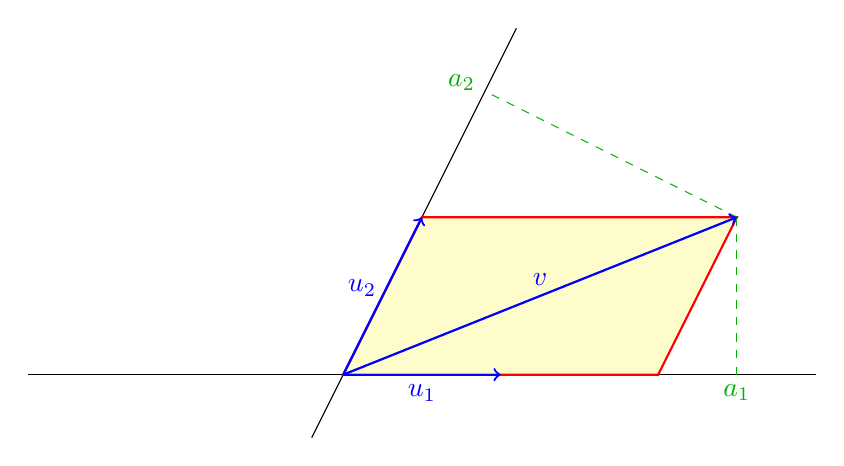
\begin{tikzpicture}[scale=2]
    \draw (-2,0) -- (3,0);
    \draw (-0.2,-0.4) -- (1.1,2.2);
    \draw[thick,red,fill=yellow!20] (0,0) -- (2,0) -- (2.5,1) -- (0.5,1) -- cycle;
    \draw[dashed,green!70!black] (2.5,1) -- (2.5,0) node[below]{$a_1$};
    \draw[dashed,green!70!black] (2.5,1) -- (0.9,1.8) node[left,yshift=3]{$a_2$};
    \draw[thick,blue,->] (0,0) -- node[below]{$\vect{u}_1$} (1,0);
    \draw[thick,blue,->] (0,0) -- node[left, pos=0.55]{$\vect{u}_2$} (0.5,1);
    \draw[thick,blue,->] (0,0) -- node[above]{$\vect{v}$} (2.5,1);
  \end{tikzpicture}
